\documentclass[12pt,a4paper]{article}

\renewcommand*\contentsname{Sadržaj}
\renewcommand{\figurename}{Slika}

\usepackage[margin=0.85in]{geometry}
\usepackage{graphicx}
\usepackage{subcaption}
\usepackage{float}
\usepackage{listings}
\usepackage{amsmath}
\usepackage{hyperref}

% Default fixed font does not support bold face
\DeclareFixedFont{\ttb}{T1}{txtt}{bx}{n}{12} % for bold
\DeclareFixedFont{\ttm}{T1}{txtt}{m}{n}{12}  % for normal

% Custom colors
\usepackage{color}
\definecolor{deepblue}{rgb}{0,0,0.5}
\definecolor{deepred}{rgb}{0.6,0,0}
\definecolor{deepgreen}{rgb}{0,0.5,0}

% Python style for highlighting
\newcommand\pythonstyle{\lstset{
language=Python,
basicstyle=\ttm,
otherkeywords={self},             % Add keywords here
keywordstyle=\ttb\color{deepblue},
emph={MyClass,__init__},          % Custom highlighting
emphstyle=\ttb\color{deepred},    % Custom highlighting style
stringstyle=\color{deepgreen},
frame=tb,                         % Any extra options here
showstringspaces=false            % 
}}


% Python environment
\lstnewenvironment{python}[1][]
{
\pythonstyle
\lstset{#1}
}
{}

% Python for external files
\newcommand\pythonexternal[2][]{{
\pythonstyle
\lstinputlisting[#1]{#2}}}

% Python for inline
\newcommand\pythoninline[1]{{\pythonstyle\lstinline!#1!}}

\renewcommand{\arraystretch}{1.5}
\begin{document}

\begin{titlepage}
	\centering
	{\scshape Univerzitet u Sarajevu \par}
	{\scshape Elektrotehnički Fakultet \par}
	\vspace{1cm}
	{\Large\scshape Prepoznavanje Oblika i Obrada Slike\par}
	\vspace{1.5cm}
	{\huge\bfseries Projektni Zadatak br. 3\par}
	\vspace{2cm}
	\Large Studenti: \par
	{\Large\itshape \textsc{Muftić} Belma, 1423/17260\par}
	{\Large\itshape \textsc{Lemeš} Lamija, 1474/17070\par}
	{\Large\itshape \textsc{Krupalija} Ehlimana, 1431/17461\par}
	\vfill
	Odgovorni asistent:\par
	MoE \textsc{Sumejja Porča}
	\vfill
	{\large Decembar, 2018\par}
\end{titlepage}

\pagenumbering{gobble}

\tableofcontents

\newpage

\pagenumbering{arabic}
\setcounter{page}{1}

\section{Prepoznavanje oblika}

\subsection{Koraci prije detekcije}

Detekcija oblika ćelije implementirana je u okviru \textit{file}-a \texttt{main.py} koji se nalazi u folderu \textit{Code}. Ta funkcija kao parametar prima \textit{folder} u kojem se nalaze slike koje je potrebno detektovati, kao i najveći broj u imenu slika koje se nalaze u njemu.

Nakon što se sa \textit{pickle} učita prethodno kreirani model, potrebno je obraditi slike tako da se deskriptor može kreirati. Slike se nalaze u folderu \textit{Validacija}, te kako je \textit{dataset} inicijalno imao 90 slika, 10 slika je spadalo u validaciju. Kako su se nasumice birale slike, potrebno je kod staviti u \texttt{try-except} blok, u slučaju da se naiđe na sliku koja se ne nalazi u \textit{folder}u. Na osnovu karakteristike da je posmatrana ćelija tamnije obojena u odnosu na ostale ćelije, koristi se \texttt{inRange} da se kreira maska, nakon čega se primjeni morfologija da se uklone regije koje su se slučajno našle u zadatom rasponu. Tako kreirana maska se šalje kao parametar u funkciju \texttt{HuMoments} da se kreira deskriptor, nakon čega se sa modelom testira kojoj klasi ćelija pripada.\\
~\\
Navedene funkcionalnosti implementirane su na sljedeći način:\\

\pythonexternal{main.py}

\newpage

\subsection{Detekcija}

Da bi se izvršila detekcija, potrebno je pronaći sve konture prethodno kreirane binarne slike, nakon čega se konture sortiraju po veličini, da bi se na prvom mjestu našla ona kontura koja opisuje ćeliju. Uz pomoć \texttt{boundingRect} moguće je pronaći kvadrat koji se nalazi oko zadane konture, te se isti nacrta. Rezultat testiranja modela se uz pomoć \texttt{putText} napiše u gornjem lijevom uglu slike, te se tako modifikovana slika prikaže korisniku. \\
~\\
Na sljedećim slikama prikazan je rezultat pokretanja detekcije nad nekoliko slika:

\begin{figure}[H]
\begin{subfigure}{.5\textwidth}
  \centering
  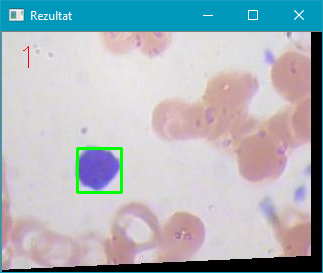
\includegraphics[scale=.9]{slikaMain1.png}
  \caption{Detektovana ćelija: \textit{Lymphocyte}}
\end{subfigure}
\begin{subfigure}{.5\textwidth}
  \centering
  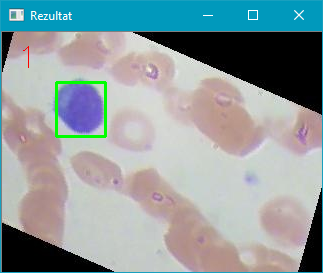
\includegraphics[scale=.9]{slikaMain2.png}
  \caption{Detektovana ćelija: \textit{Lymphocyte}}
\end{subfigure}
\begin{subfigure}{.5\textwidth}
  \centering
  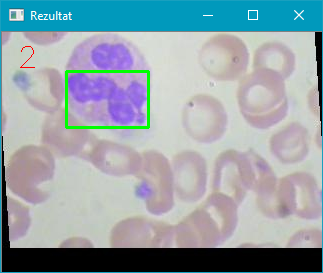
\includegraphics[scale=.9]{slikaMain3.png}
  \caption{Detektovana ćelija: \textit{Neutrophil}}
\end{subfigure}
\begin{subfigure}{.5\textwidth}
  \centering
  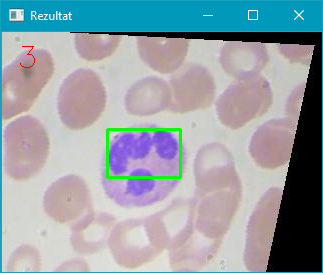
\includegraphics[scale=.9]{slikaMain4.png}
  \caption{Detektovana ćelija: \textit{Something else}}
\end{subfigure}
\caption{Rezultati detekcije nad slikama za validaciju}
\end{figure}

\newpage

\subsection{Korištenje \textit{slider}-a}

\textit{Slider} je objekat koji izvršava podjelu slike na isječke koji se zatim pojedinačno testiraju koristeći prethodno opisane koncepte. Ovaj objekat ima sljedeće atribute:

\begin{itemize}
\renewcommand\labelitemi{--}
\item \texttt{windowSize}: veličina prozora, odnosno kvadrata koji predstavlja isječak slike;
\item \texttt{step}: korak, odnosno veličina koja određuje za koliko će se prozor pomjeriti (jednak i za visinu, i za širinu);
\item \texttt{scaleChange}: veličina koja određuje koliko će se puta povećati prozor nakon što se dođe do kraja slike (ukoliko skaliranje bude neophodno);
\item \texttt{imageSize}: veličina slike, koja određuje do kojih koordinata će se kretati vrijednosti koje određuju prozor;
\item \texttt{coordinates}: koordinate vrhova kvadrata, neophodne za kreiranje isječaka slike;
\item \texttt{maxScale}: maksimalni broj puta povećanja prozora (maksimalno skaliranje);
\item \texttt{currentScale}: broj puta povećavanja prozora (broj skaliranja);
\item \texttt{willScale}: veličina koja određuje da li će se skaliranje vršiti, te koja je postavljena na \texttt{True}, osim u slučaju da se objekat detektuje na slici.

\end{itemize}

Funkcija \texttt{slide} vrši pomijeranje prozora, dok funkcija \texttt{oneSlide} vrši pravljenje isječka slike. Nakon što se prozor pomjeri i isječak kreira, vrši se detekcija na način kako je to prethodno opisano.\\

Ukoliko se ni u jednom isječku ne izvrši pozitivna detekcija, vrši se skaliranje, te se cijeli postupak zatim ponavlja. Ukoliko se ne detektuje nijedan objekat na slici, jednostavno se nastavlja s detekcijom na sljedećoj slici. Ukoliko dođe do detekcije, na slici se prikazuje pravougaonik koji se sastoji od svih isječaka na kojima je izvršena detekcija. Budući da je moguće da se detektuje više različitih vrsta oblika na slici (ukoliko se objekat nađe u više isječaka), konačni rezultat predstavlja ona klasa za koju je detektovano najviše isječaka.\\

\newpage

Na sljedećim slikama prikazan je rezultat pokretanja detekcije nad nekoliko slika:

\begin{figure}[H]
\begin{subfigure}{.5\textwidth}
  \centering
  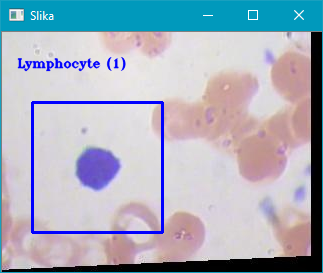
\includegraphics[scale=.9]{slikaSlider1.png}
  \caption{Detektovana ćelija: \textit{Lymphocyte}}
\end{subfigure}
\begin{subfigure}{.5\textwidth}
  \centering
  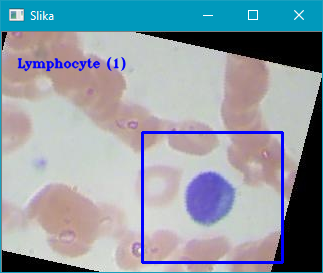
\includegraphics[scale=.9]{slikaSlider2.png}
  \caption{Detektovana ćelija: \textit{Lymphocyte}}
\end{subfigure}
\begin{subfigure}{.5\textwidth}
  \centering
  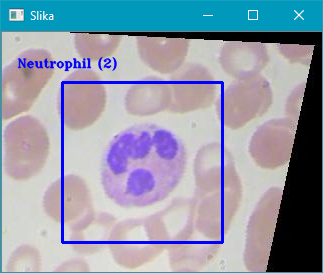
\includegraphics[scale=.9]{slikaSlider3.png}
  \caption{Detektovana ćelija: \textit{Neutrophil}}
\end{subfigure}
\begin{subfigure}{.5\textwidth}
  \centering
  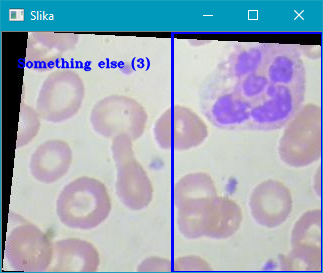
\includegraphics[scale=.9]{slikaSlider4.png}
  \caption{Detektovana ćelija: \textit{Something else}}
\end{subfigure}
\caption{Rezultati detekcije nad slikama za validaciju uz korištenje \textit{slider}-a}
\end{figure}

\end{document}